\documentclass[11pt]{article}
\usepackage[margin=2.6cm]{geometry}
\usepackage{graphicx,booktabs,amsmath,xcolor}
\usepackage[colorlinks=true,linkcolor=blue!50!black,citecolor=blue!50!black,urlcolor=blue!50!black]{hyperref}
\usepackage{caption}
\captionsetup{font=small,labelfont=bf,justification=justified}
\newcommand{\pt}{\ensuremath{p_\mathrm{T}}}
\newcommand{\pttrue}{\ensuremath{p_\mathrm{T}^\mathrm{true}}}
\newcommand{\ptreco}{\ensuremath{p_\mathrm{T}^\mathrm{reco}}}
\graphicspath{{figures/}}

\title{\vspace{-1.2cm}{\color{red!70!black}\small\bfseries INTERNAL DRAFT --- UTA DFM GROUP --- NOT AN OFFICIAL ATLAS DOCUMENT}\\[2mm]
\Large Machine-Learned Jet \pt{} Calibration from Low-Level Detector Information\\[1mm]
\normalsize DFM-NOTE-2026-01}
\author{\small UTA Detector Foundation Model group\\
\small (A.~Farbin, M.~A.~Ghaznavi, U.~Ghaznavi et al.; analysis assisted by Claude)}
\date{\small August 2026 \;\textbullet\; \texttt{github.com/afarbin/DetectorFoundationModel}, branch \texttt{dfm-merge}}

\begin{document}
\maketitle

\begin{abstract}
We present a systematic study of machine-learned jet transverse-momentum calibration
from low-level detector information, using 620k truth-matched light jets from simulated
$t\bar t$ events. A shared token encoder over calorimeter cells (with the detector
neighbor graph recovered via exact cell matching between two ntuple formats), charged
tracks, and reconstructed jet features is trained to regress the per-jet log \pt{}
response with a heteroscedastic Gaussian objective. We compare all input combinations,
graph versus set encodings of the calorimeter, and self-supervised masked-cell
pretraining against from-scratch training. The best configuration (tracks + jet
features + cells on the neighbor graph) approximately halves the jet energy resolution
relative to the input reconstructed jets (11.9\% versus 23.8\% inclusive). Detector
topology is a measurable inductive bias for cells-only models; combining all modalities
requires $\mathcal{O}(10^5)$ labeled jets to pay off. A linear probe of the pretrained
encoder matches full end-to-end training, demonstrating that the masked-cell pretext
learns calibration-relevant representations; label-efficiency gains from pretrained
initialization are small but consistent below 10\% label fractions.
\end{abstract}

\section{Introduction}
This note is the first of three~\cite{note2,note3} documenting the initial physics
program of the UTA Detector Foundation Model (DFM) effort, which unifies two previously
separate model lines---a calorimeter-cell graph network for topoclustering
(M.~A.~Ghaznavi) and a track-based attention model for event-level $b$-tagging
(U.~Ghaznavi)---into a single shared backbone with task-specific heads (the
\texttt{dfm} package). Hadronic jet calibration was selected as the first benchmark
task following the program review~\cite{reviews}: it is a regression with unambiguous
truth, a strong classical baseline (the ATLAS jet energy scale chain~\cite{topoclus}),
and it exercises every component of the merged architecture.

The target throughout is the per-jet log response
$y=\ln(\pttrue/\ptreco)$; the model predicts $(\mu,\sigma)$ per jet, and the
multiplicative correction $e^{\mu}$ defines the calibrated jet. The study is organized
in gated tiers: dataset QA and no-training baselines (Tier~0), single-input models
(Tier~1), input combinations and protocol cross-checks (Tier~2), the full-data matrix
(Tier~3), and self-supervised pretraining (Tier~4).

\section{Data samples and the cell-matching bridge}
Two ntuple formats enter the study. The \textbf{5D ntuples} (17 files, 340k simulated
$t\bar t$ events) provide tracks, jets, truth information, and a \emph{thinned}
calorimeter cell record; we measured the thinning empirically to be a per-cell
threshold $E>0.5$\,GeV and $E>2\sigma_\text{noise}$, positive energies only. The
\textbf{Calo ntuples} provide all 187{,}652 calorimeter cells per event in fixed hash
order with the full detector neighbor list, plus topocluster associations.

The two formats contain different event samples, but their cell centres are
bit-identical: an exact nearest-neighbour match in $(x,y,z)$ within sampling layer
(library \texttt{cell\_matching.py}) identifies every 5D cell with its calorimeter
hash position with zero mismatches in 146k jets tested, and a persistent Cell-ID
lookup makes this free after warm-up. This bridge transfers the \emph{detector
neighbor graph} onto the thinned 5D cells---enabling the graph-encoding comparisons of
this note---and connects the pretraining corpus (Calo format) to the calibration data
(5D format).

The thinned cell record retains 75.0\% of the energy of the cells in jets
($\pt>20$\,GeV; per-jet median 63\%, 10th--90th percentile 32--85\%, rising with jet
energy), with strong layer dependence (EMB1/EMB3 $\sim$33\%, Tile A/BC 81--86\%).
Cells-only results below are therefore lower bounds on full-cell performance. Large
negative deposits in the forward calorimeter (FCAL pileup noise reaches tens of GeV
per cell, and out-of-time pileup produces negative event sums) are handled with a
cell-level $|E|<100$\,GeV cut rather than event vetoes; jet cones are central and
unaffected.

\section{Per-jet dataset}
One sample per truth-matched light jet (\texttt{HadronConeExclTruthLabelID}=0):
$\pttrue>20$\,GeV, recomputed $\Delta R(\text{reco},\text{truth})<0.3$, $|\eta|<2.5$,
duplicate-truth-match removal. Isolation (no reco jet with $\pt>15$\,GeV within
$\Delta R<0.8$; no other truth match within $\Delta R<1.0$) is stored as a flag:
training uses isolated jets, and both populations are evaluated separately. Per jet we
store: 6 jet features; all ghost-associated tracks with 18 features each (kinematics,
impact-parameter significances computed from the track covariances, hit content); all
cone ($\Delta R<0.4$) cells with the 7-feature calorimeter schema and their matched
neighbor subgraph; and metadata. Splits are by file: 13 train / 2 validation / 2 test
files $=$ 181k isolated training jets of 620k total. Training weights flatten the
\pttrue{} spectrum over 20--250\,GeV (capped at the 99th percentile).

\section{Methodology}
\subsection{Model}
All configurations are assemblies of the shared \texttt{dfm} backbone: per-modality
input projections with type embeddings; local mixing per modality (SAGE-style
convolution over the fixed calorimeter neighbor subgraph for cells; masked $k$-NN
EdgeConv in $(\eta,\sin\phi,\cos\phi)$ for tracks); a shared mask-aware
induced-set-attention (ISAB) stack, cross-modality where multiple inputs are present;
masked-mean global pooling; and a head MLP emitting $(\mu,\log\sigma^2)$. Jet
features, when enabled, join at the head. Models are ${\sim}1$M parameters (dim 128,
2 local + 2 global layers)---deliberately small, as the study compares information
content, not capacity.

\subsection{Training and metrics}
Loss: Huber warm-up (5 epochs) then heteroscedastic Gaussian NLL; AdamW with cosine
schedule; early stopping on validation NLL; 3 seeds per configuration. Metrics per
$(\pttrue,|\eta|,\phi)$ bin on the corrected response
$r_\text{corr}=(\ptreco/\pttrue)\,e^{\mu}$: \textbf{JES closure} $=$
median$(r_\text{corr})$ (target $\pm 1$--2\%); \textbf{JER} $=$
$(q_{75}-q_{25})/1.349\div\text{median}$ (Gaussian-equivalent robust width);
\textbf{pull} $=(y-\mu)/\sigma$ (unit-normal if $\sigma$ is calibrated). Baselines:
B0 $=$ the ntuple's calibrated jets after our cuts; B1 $=$ one global median
correction; B2 $=$ the jet-features-only model.

\section{Results}
\subsection{Tier 0 --- the uncorrected picture}
\begin{figure}[htbp]\centering
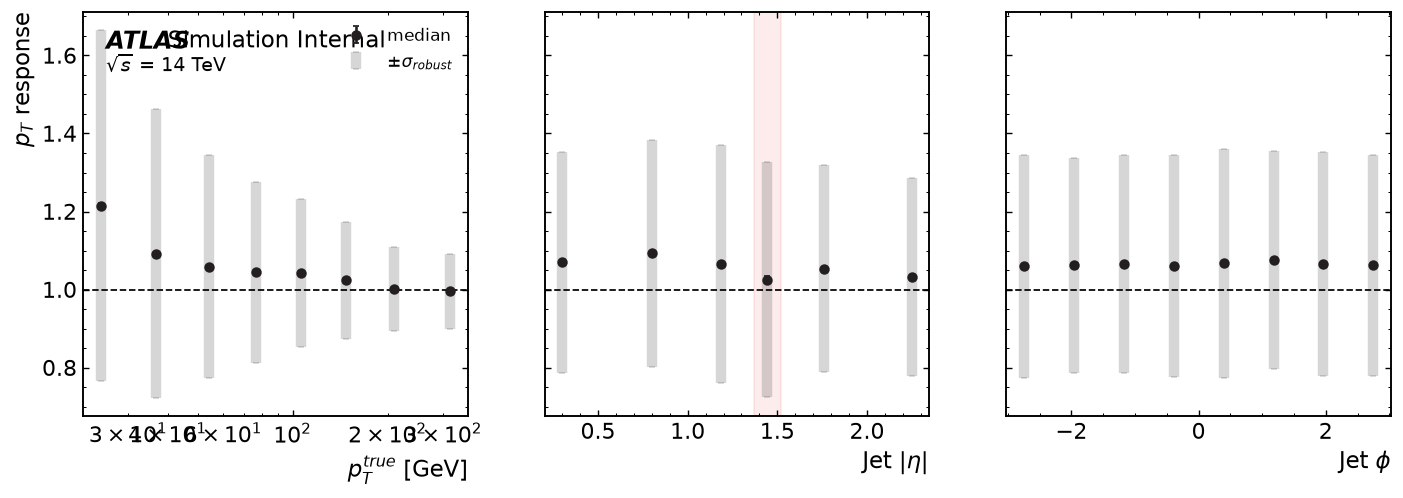
\includegraphics[width=\textwidth]{H3_b0_profiles.png}
\caption{Uncorrected (B0) response versus \pttrue, $|\eta|$ (crack band shaded), and
$\phi$: median with statistical errors and the robust $\pm\sigma$ band. The input jets
read $+21\%$ high at 20--30\,GeV, falling to unity above 150\,GeV; $\phi$ is flat as
required in simulation.}
\label{fig:b0}
\end{figure}
\begin{figure}[htbp]\centering
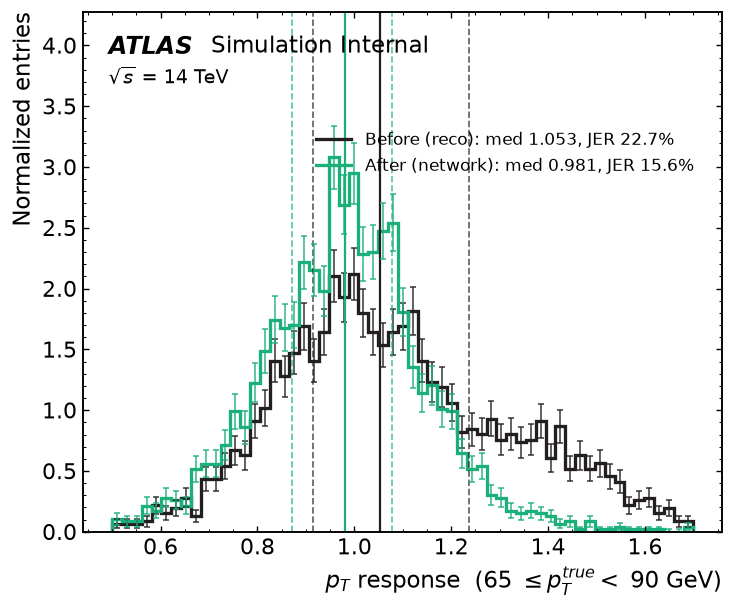
\includegraphics[width=0.62\textwidth]{H4_metric_explained.png}
\caption{The metric definitions at work in a single bin (65--90\,GeV): response before
and after correction, with medians (solid) and quartiles (dashed). The correction both
centres the median (JES) and narrows the quartile span (JER).}
\label{fig:metric}
\end{figure}

\subsection{Tiers 1--2 --- single inputs and combinations (4-file dataset)}
On the initial 4-file dataset (146k jets): the calorimeter neighbor graph beats a set
encoding of the same cells on every metric ($\Delta$NLL${}\approx 0.11$); constituent
inputs (tracks or cells) each cut JER by ${\sim}30\%$ while the jet 4-vector alone
improves resolution by exactly nothing (it can only re-centre); tracks and cells
combine (TC 0.147 versus 0.157/0.158 alone); and a median-targeting (MAE) training
variant confirmed a ${\sim}2\%$ mean-versus-median estimator offset in the NLL
closure, fixable by protocol. $\mu$-conditioning changed nothing, isolating the
jet-feature advantage as thinned-away constituent information rather than pileup
conditioning.

\begin{figure}[htbp]\centering
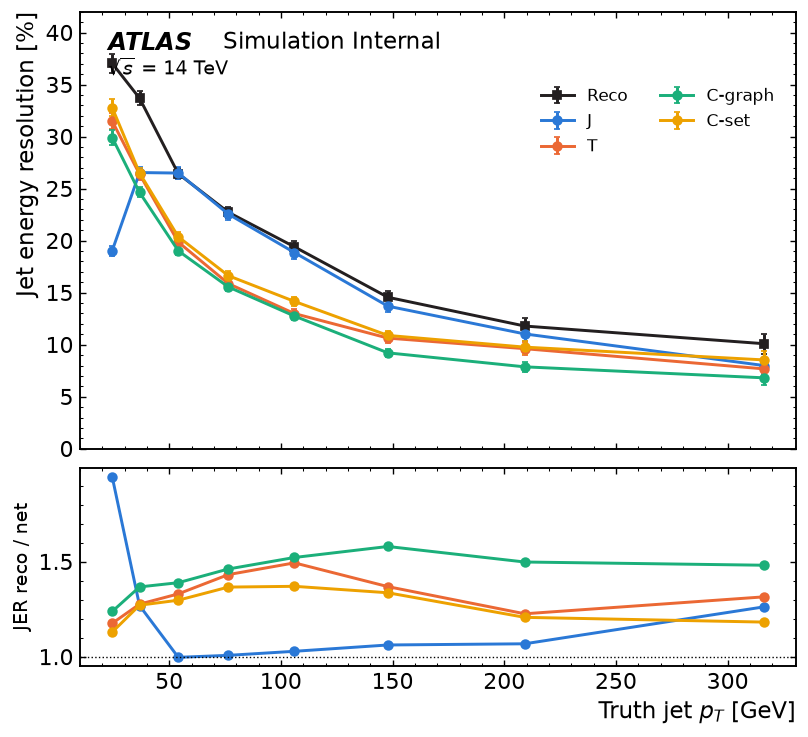
\includegraphics[width=0.72\textwidth]{U2_jer_ratio_all.png}
\caption{Tier-1 jet energy resolution versus \pt{} for all single-input configurations
with the improvement ratio (uncorrected/model) below. Note the first bin of the
jet-features-only model: narrow but at the wrong scale (closure 1.19)---regression to
the spectrum prior, and the reason closure and resolution must always be read
together.}
\label{fig:tier1jer}
\end{figure}
\begin{figure}[htbp]\centering
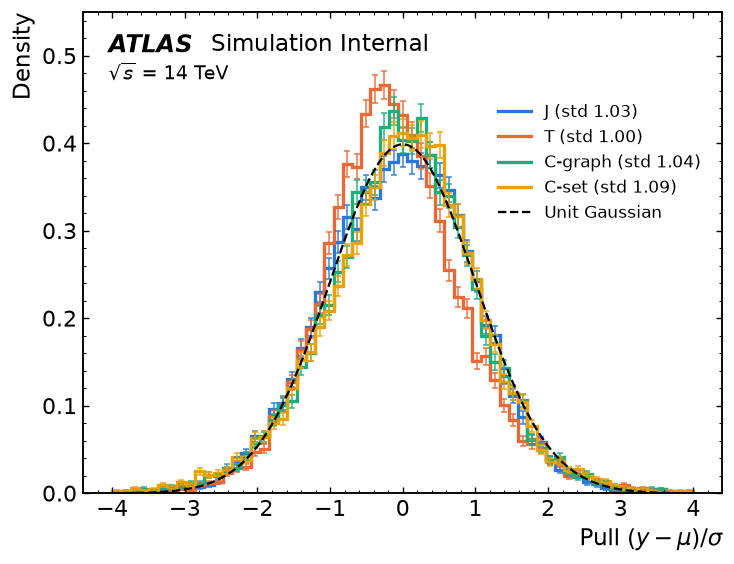
\includegraphics[width=0.6\textwidth]{H5_pulls.png}
\caption{Per-jet uncertainty validation: pull distributions against a unit Gaussian
for the Tier-1 models (std 1.03--1.05).}
\label{fig:pulls}
\end{figure}

\subsection{Tier 3 --- the full-data matrix}
Scaling to all 17 files improved every configuration and \textbf{reversed one Tier-2
conclusion}: with sufficient statistics, cells contribute on top of tracks + jet
features (Table~\ref{tab:full}, Figs.~\ref{fig:headline}--\ref{fig:fulljer}). The best
model, TJC-graph, reaches JER 0.115 at 65--90\,GeV versus 0.230 uncorrected.

\begin{table}[htbp]\centering\small
\begin{tabular}{lcccc}\toprule
configuration & NLL & MAE & closure RMS & JER@65--90\\\midrule
\textbf{TJC-graph} & $\mathbf{-1.422}$ & \textbf{0.124} & 4.0\% & \textbf{0.115}\\
TJC-set   & $-1.416$ & 0.125 & 4.2\% & 0.116\\
TJ        & $-1.364$ & 0.130 & 4.5\% & 0.125\\
TC-graph  & $-1.241$ & 0.153 & 4.4\% & 0.130\\
T         & $-1.058$ & 0.175 & \textbf{3.0\%} & 0.150\\
C-graph   & $-1.086$ & 0.174 & 6.9\% & 0.158\\
B0 uncorrected & --- & --- & --- & 0.230\\\bottomrule
\end{tabular}
\caption{Full-data results, isolated test jets, mean of 3 seeds.}
\label{tab:full}
\end{table}

\begin{figure}[htbp]\centering
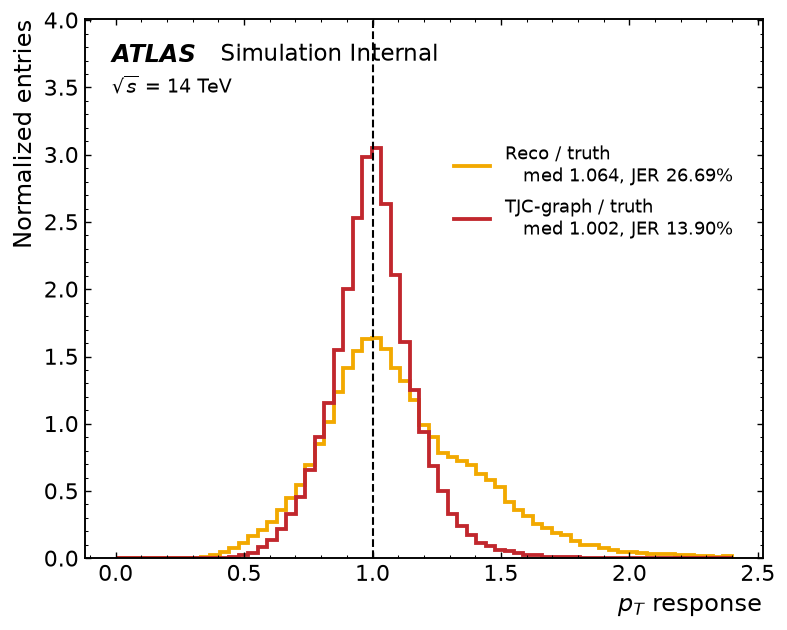
\includegraphics[width=0.6\textwidth]{FF6_headline_response.png}
\caption{Headline result: inclusive \pt{} response of the best model (TJC-graph)
versus the input reconstructed jets---resolution approximately halved (11.9\% vs
23.8\%) with median response 1.00.}
\label{fig:headline}
\end{figure}
\begin{figure}[htbp]\centering
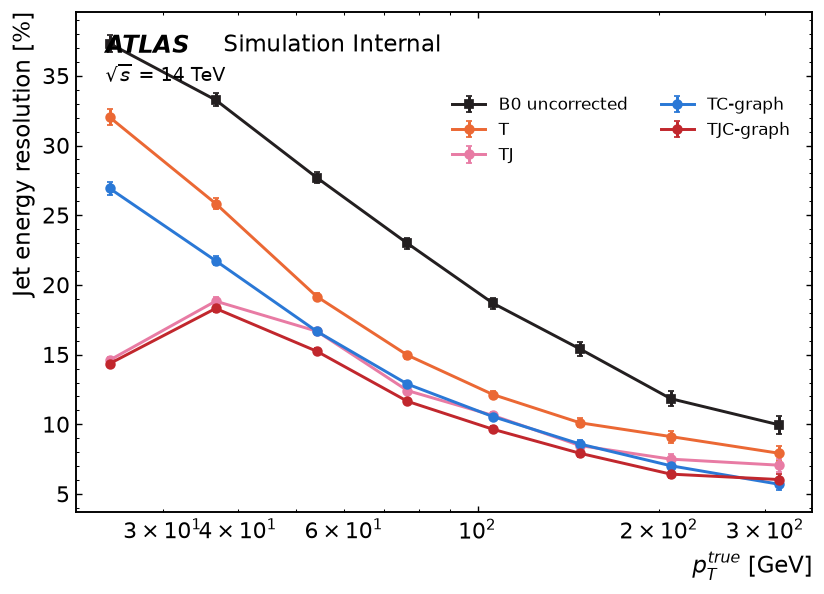
\includegraphics[width=0.68\textwidth]{FF1_jer.png}
\caption{Full-data JER versus \pt{} for the key configurations: every addition of
detector information helps, across the full spectrum.}
\label{fig:fulljer}
\end{figure}

\subsection{Tier 4 --- self-supervised pretraining}
Masked-cell pretraining (cluster masking at ratio 0.15, reconstructing the scaled cell
significance, with a mask-indicator channel making pretrained and finetuned encoders
weight-compatible) was performed on all three processed calorimeter corpora
($t\bar t$ + single-pion + $hh\to bb\tau\tau$, 14.4k events); scaling the corpus
16$\times$ improved validation reconstruction from 0.507 to 0.347. Transfer results
(Table~\ref{tab:pre}, Figs.~\ref{fig:labeleff}--\ref{fig:preqa}): finetuning from the
pretrained encoder neither helps nor hurts at full labels; the \textbf{linear
probe}---frozen encoder, trained head---matches full end-to-end training (JER 0.157
vs 0.158) with the best closure of its family; and pretrained initialization is
consistently ${\sim}1$--2\% relatively better at 1\% and 10\% label fractions.

\begin{table}[htbp]\centering\small
\begin{tabular}{lccc}\toprule
C-graph variant & NLL & closure RMS & JER@65--90\\\midrule
from scratch & $-1.086$ & 6.9\% & 0.158\\
pretrained + finetune & $-1.086$ & 6.2\% & 0.158\\
linear probe (frozen) & $-1.041$ & \textbf{5.7\%} & 0.157\\\bottomrule
\end{tabular}
\caption{Pretraining transfer, cells-only model.}
\label{tab:pre}
\end{table}

\begin{figure}[htbp]\centering
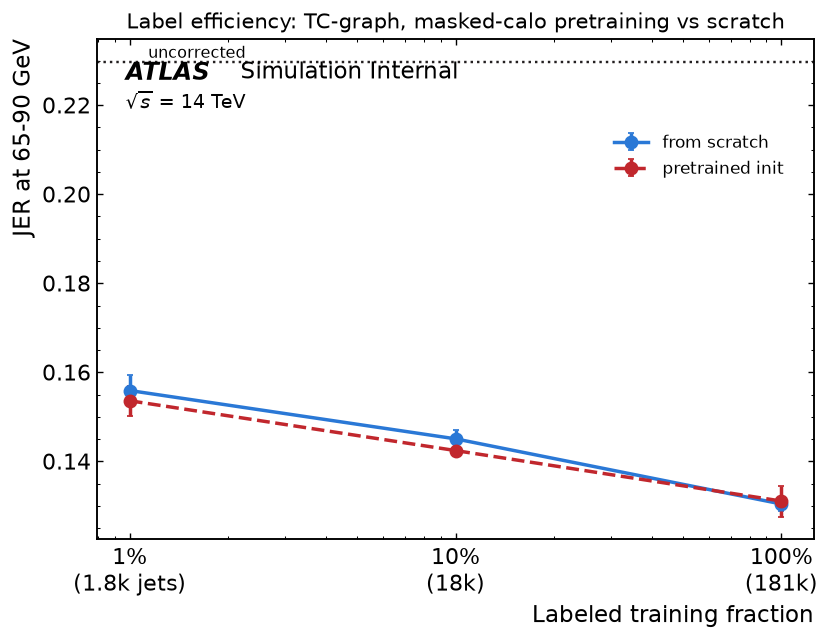
\includegraphics[width=0.62\textwidth]{FF3_label_efficiency.png}
\caption{Label efficiency: JER at 65--90\,GeV versus labeled training fraction for
TC-graph from scratch (blue) and from pretrained initialization (red dashed).}
\label{fig:labeleff}
\end{figure}
\begin{figure}[htbp]\centering
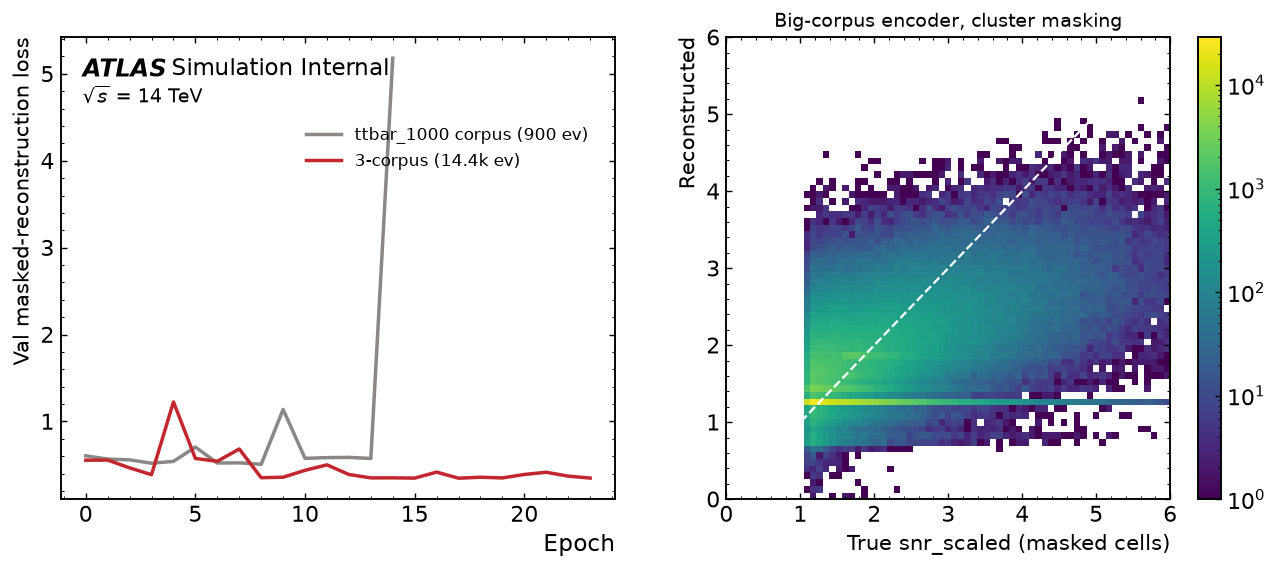
\includegraphics[width=\textwidth]{FF5_pretrain_qa.png}
\caption{Pretraining QA: validation masked-reconstruction loss for the small and
3-corpus pretrainings (left); reconstructed versus true masked-cell significance for
the big-corpus encoder (right).}
\label{fig:preqa}
\end{figure}

\section{Systematic considerations and known limitations}
\begin{itemize}
\item \textbf{Cell thinning}: the 5D subset carries 75\% of jet cell energy with a
fluctuating jet-by-jet deficit; cells-only numbers are lower bounds.
\item \textbf{Truth-match purity}: rests on the recomputed $\Delta R<0.3$ and
$\pttrue>20$\,GeV cuts, validated by the B0 response tightening to median 1.065.
\item \textbf{Low-\pt{} closure}: no configuration closes the 20--30\,GeV bin
(spectrum-edge migration); numerical inversion is the designated fix, together with
the MAE/median protocol for the ${\sim}2\%$ NLL estimator offset.
\item \textbf{Sample dependence}: single $t\bar t$ sample; event-level context learned
by the models is legitimate physics but sample-specific.
\item \textbf{Pretraining overlap}: event disjointness between the $t\bar t$
pretraining corpus and the 5D files is unverifiable; the 3-corpus mix dilutes, and the
probe result is immune in interpretation.
\item \textbf{Isolation}: headline numbers are for isolated jets; the measured
isolated$\to$non-isolated degradation defines the target for event-level Stage 2.
\end{itemize}

\section{Conclusions}
A shared token encoder over thinned calorimeter cells, tracks, and jet features---with
the detector neighbor graph recovered by exact cell matching---halves the jet \pt{}
resolution of the input reconstruction across 20--400\,GeV while closing the scale to
a few percent. Detector topology is a real inductive bias for calorimeter-only models;
full input combination pays off once $\mathcal{O}(10^5)$ labeled jets are available.
The masked-cell pretext demonstrably learns calibration-relevant representations
(probe $\approx$ full training), with small consistent label-efficiency gains at this
model scale. These results establish the baseline and machinery for the flavor-aware
studies of Ref.~\cite{note2} and the joint tagging--calibration study of
Ref.~\cite{note3}.

\appendix
\section{Operations}
The campaign (41 trainings + 2 pretrainings, $4\times$A30) survived one node freeze
requiring an administrator reboot. Root cause: uncapped torch/numpy OpenMP thread
pools (56 threads per process, stacked across concurrent jobs starving the scheduler);
mitigations now standard: thread caps, niced processes, an alert/pause/kill resource
watchdog, SSH connection multiplexing, reboot-proof code and state locations, and
re-entrant job queues.

\begin{thebibliography}{9}
\bibitem{note2} DFM-NOTE-2026-02, \emph{Flavor-Dependent Machine-Learned Jet
Calibration}, \texttt{notes/DFM-NOTE-2026-02-flavor-calibration/}.
\bibitem{note3} DFM-NOTE-2026-03, \emph{Panoptic Flavor Tagging and Jet Calibration},
\texttt{notes/DFM-NOTE-2026-03-panoptic-tagging-calibration/}.
\bibitem{reviews} A.~Farbin, \emph{CaloGraphNet reviews},
\texttt{reviews/calographnet\_review.md},
\texttt{reviews/btagging\_masking\_review.md} (2026).
\bibitem{topoclus} ATLAS Collaboration, \emph{Topological cell clustering in the ATLAS
calorimeters}, arXiv:1603.02934, and the JES chain references therein.
\end{thebibliography}
\end{document}
